
\PassOptionsToPackage{full}{textcomp}
\documentclass[]{tufte-handout}
%\usepackage{fontspec}
%\usepackage{ETbb}


% load babel package and options here
%\usepackage[p,osf]{ETbb} % osf in text, tabular lining figures in math
\usepackage{ETbb} % osf in text, tabular lining figures in math
\usepackage[scaled=.95,type1]{cabin} % sans serif in style of Gill Sans
\usepackage[varqu,varl]{zi4}% inconsolata typewriter
\usepackage[T1]{fontenc} % LY1 also works
\usepackage[libertine,vvarbb]{newtxmath}
%\usepackage[cal=boondoxo,bb=boondox,frak=boondox]{mathalfa}

%\geometry{showframe} % display margins for debugging page layout

\usepackage{graphicx} % allow embedded images
%  \setkeys{Gin}{width=\linewidth,totalheight=\textheight,keepaspectratio}
  \graphicspath{{graphics/}} % set of paths to search for images
\usepackage{amsmath}  % extended mathematics
\usepackage{booktabs} % book-quality tables
%\usepackage{units}    % non-stacked fractions and better unit spacing
\usepackage{multicol} % multiple column layout facilities
\usepackage{multirow} % multiple column layout facilities
\usepackage{lipsum}   % filler text
\usepackage{fancyvrb} % extended verbatim environments
  \fvset{fontsize=\normalsize}% default font size for fancy-verbatim environments
\usepackage{gensymb} % provides symbols like \degree
\usepackage{ragged2e} % enables hyphenation in ragged-right justification
\usepackage[normalize-symbols]{textalpha} %enables \textalpha for alpha symbol etc.

\usepackage{hyperref} % enables styling of href and url
\hypersetup{
    pdftitle={Tutorial X},
    pdfauthor={Barry Linkletter},
    colorlinks=true,
    linkcolor=blue,
    filecolor=magenta,      
    urlcolor=blue,
    pdfborder={0 0 0},
    frenchlinks=false,
    pdfpagemode=FullScreen,
    }

\usepackage{enumitem} % allows resuming enumerate lists.
\usepackage{mathtools}
\usepackage{mhchem}

\usepackage{siunitx} % provides "S" column class for aligning decimals.  


\usepackage{nicefrac}

\usepackage{varioref}

\usepackage{babel}
\usepackage{float}
\usepackage{stackrel}


\usepackage[shortconst]{physconst}

\usepackage[normalem]{ulem}  % provides strikethrough \sout{}

\usepackage{newfloat}
\DeclareFloatingEnvironment[
  fileext = los ,
  listname = {List of Schemes} ,
  name = Scheme
]{scheme}                    % provides scheme numbering for chemical schemes



\newcommand{\Km}{$\rm K_M$}
\newcommand{\Vmax}{$\rm V_{max}$}
\newcommand{\kcat}{$\rm k_{cat}$}



\title{Tutorial \#X: Preminary Report}
\author[Barry Linkletter]{Barry Linkletter}
\date{} % without \date command, current date is supplied


\begin{document}
\justifying


\maketitle% this prints the handout title, author, and date

\begin{abstract}
\noindent This is the final report produced by your unfortunate predecessor. It describes the enzyme assays for wild-type \emph{\textbeta -galactosidase} with PNP-\textbeta-D-Gal. Please use this report to develop your own method for analyzing the remaining data that still needs to be analyzed. Then you may have cake.
\marginnote[-20mm]{This document was produced using the \LaTeX\ typesetting language with the Tufte-handout document class. Images of proteins were created using \textit{UCSF Chimera}. Chemical diagrams were made with \textit{ChemDoodle} and further edited with \textit{Affinity Designer}.}

\end{abstract}





\section{Part 1: Introduction}

This report describes the data analysis for the enzyme assay used to evaluate mutated \emph{\textbeta -galactosidase} enzymes. First we must determine and enzyme conc\-en\-trat\-ion that will give reaction rates that are fast enough to be easily followed but no too fast where we cannot collect enough data to determine an initial rate. 

\subsection{The Plate Plan}

We will evaluate three different concentrations of enzyme. The plate will be set up with eight rows of differing substrate concentration in \qty{0.100}{M} phosphate buffer. Three rows will contain no enzyme, three will have an enzyme concentration of \qty{1}{nM} and there will be two sets of three columns with dilutions of that concentration. In the first trial we will use 2-fold dilutions. The plate plan is sketched in figure~\ref{fig:fig1}.



\begin{marginfigure}[5mm]

  \caption[0mm]{The natural products daidzin and daidzein compared to our synthetic target, 7-(\textbeta -D-Galactopyranosyloxy)-4'-hydroxyisoflavone} 
  \vspace{2mm}
    \centering
  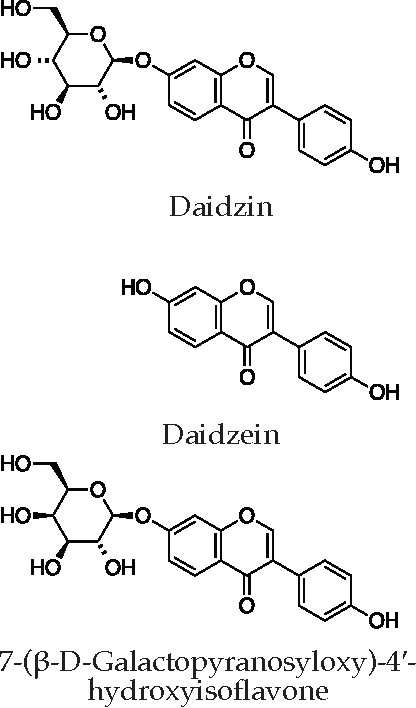
\includegraphics[scale=0.6]{Daidzin2.pdf}
  \vspace{5mm}
  \label{fig:fig1}
\end{marginfigure}



\nobibliography{}

\end{document}